\chapter{Реализация комплекса}

Курс разработан так, чтобы выполнять его можно было с любой операционной системы. Для работы с учебниками, надо установить Python 3 и Jypiter. Количество сторонних библиотек сведено к минимуму.

\section{IPython и Jupyter Notebook}

IPython является мощным инструментом для работы с языком Python. 

Jupyter Notebook представляет собой графическую веб-оболочку для интерактивных вычислений, кроме того это удобный инструмент для создания красивых аналитических отчетов, так как он позволяет хранить вместе код, изображения, комментарии, формулы и графики:

\begin{figure}[htbp]
	\centering
	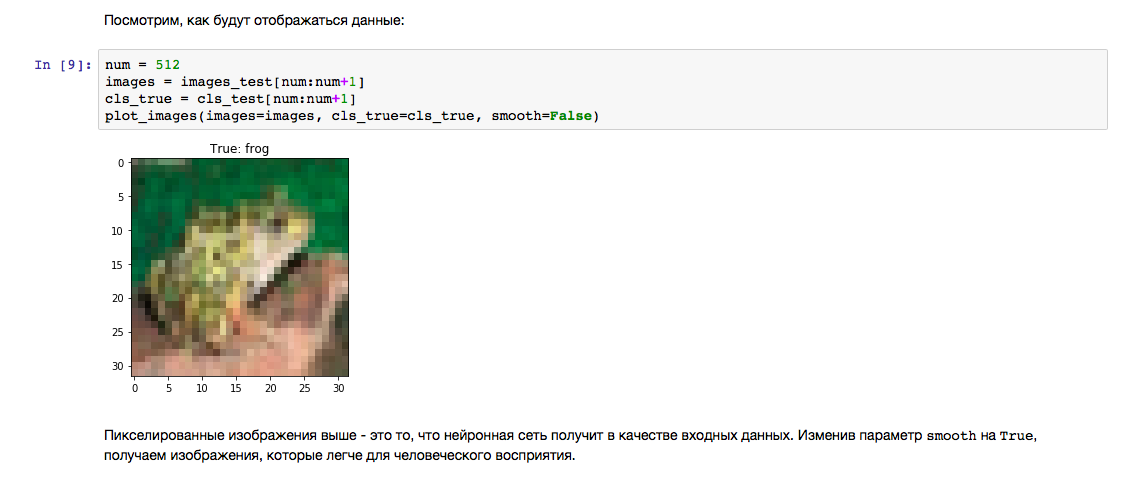
\includegraphics[width=0.9\textwidth]{fig/jn}
	\caption{Jupyter Notebook }
\end{figure}

Основные особенности этой платформы – это комплексная интроспекция объектов, сохранение истории ввода на протяжении всех сеансов, кэширование выходных результатов, магические команды, журналирование сессии, дополнительный командный синтаксис, доступ к системной оболочке. Ко всему прочему это еще и свободное программное обеспечение.

Экспортировать блокнот можно в формате IPython Notebook (.ipynb), но есть и другие варианты:
\begin{itemize}
\item преобразовать блокнот в html-файл;
\item опубликовать его в gists, где можно обрабатывать файлы этого формата;
\item сохранить блокнот на облако, а затем открыть ссылку в nbviewer&
\end{itemize}


Ко всему прочему, в блокноте есть magics-команды. Под "магией" в IPython понимаются дополнительные команды, выполняемые в рамках оболочки, которые облегчают процесс разработки и расширяют ваши возможности.

Готовые учебники - это файлы, в которых хранится исходный код, входные и выходные данные, полученные в рамках сессии. Фактически, он является записью работы, но при этом позволяет заново выполнить код. 

\section{Описание готовых работ}
В данной главе будут представлены примеры разработанных лабораторных работ  по дисциплине "исследование моделей глубокого обучения". Программы были разработаны в Jupyter Notebook на языке Python, с использованием библиотек Tensorflow и Keras.

Учебники были разработаны так, чтобы на их примере студенты смогли научиться извлекать признаки из разнородных данных, какие бывают при этом проблемы и как их решать. Также они научатся сводить задачи к формальным постановкам задачи машинного обучения и поймут, как проверять качество построенной модели на разных данных.

Пройдя этот курс, студент может получить знания о распространенных типах прикладных задач и  суметь найти схемы их решения.
 
\subsection{Структура курса}

Курс содержит три лабораторных работы, которые решают задачи: классификации, локализации изображений и прогнозирование временных рядов. 


\begin{figure}[htbp]
	\centering
	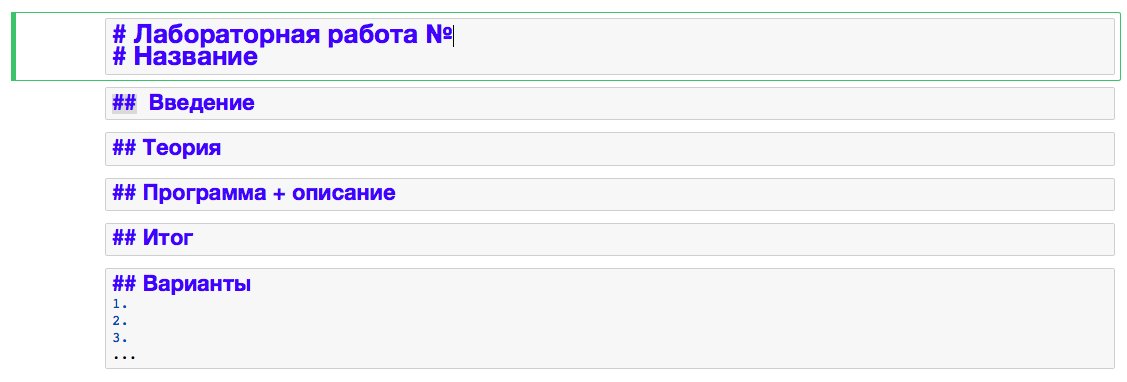
\includegraphics[width=0.7\textwidth]{fig/struct}
	\caption{Структура работ }%
	\label{fig:struct}
\end{figure}

Каждая лабораторная состоит из:
\begin{itemize}
\item название;
\item введение - краткое описание решаемых задач;
\item теорию - информацию о наборах данных, сетях, использованных в работе и алгоритмах;
\item разработанную программу и ее подробное описание;
\item итог;
\item варианты.
\end{itemize}

\subsection{Реализация первой лабораторной работы}

В разработанном учебнике показано, как создать простой классификатор изображений на основе сверточной нейронной сети и наборе данных CIFAR-10, с использованием библиотек TensorFlow и prettytensor - это прикладной интерфейс высокого уровня для TensorFlow, в разы упрощает работу с глубокими сетями.

\begin{figure}[htbp]
	\centering
	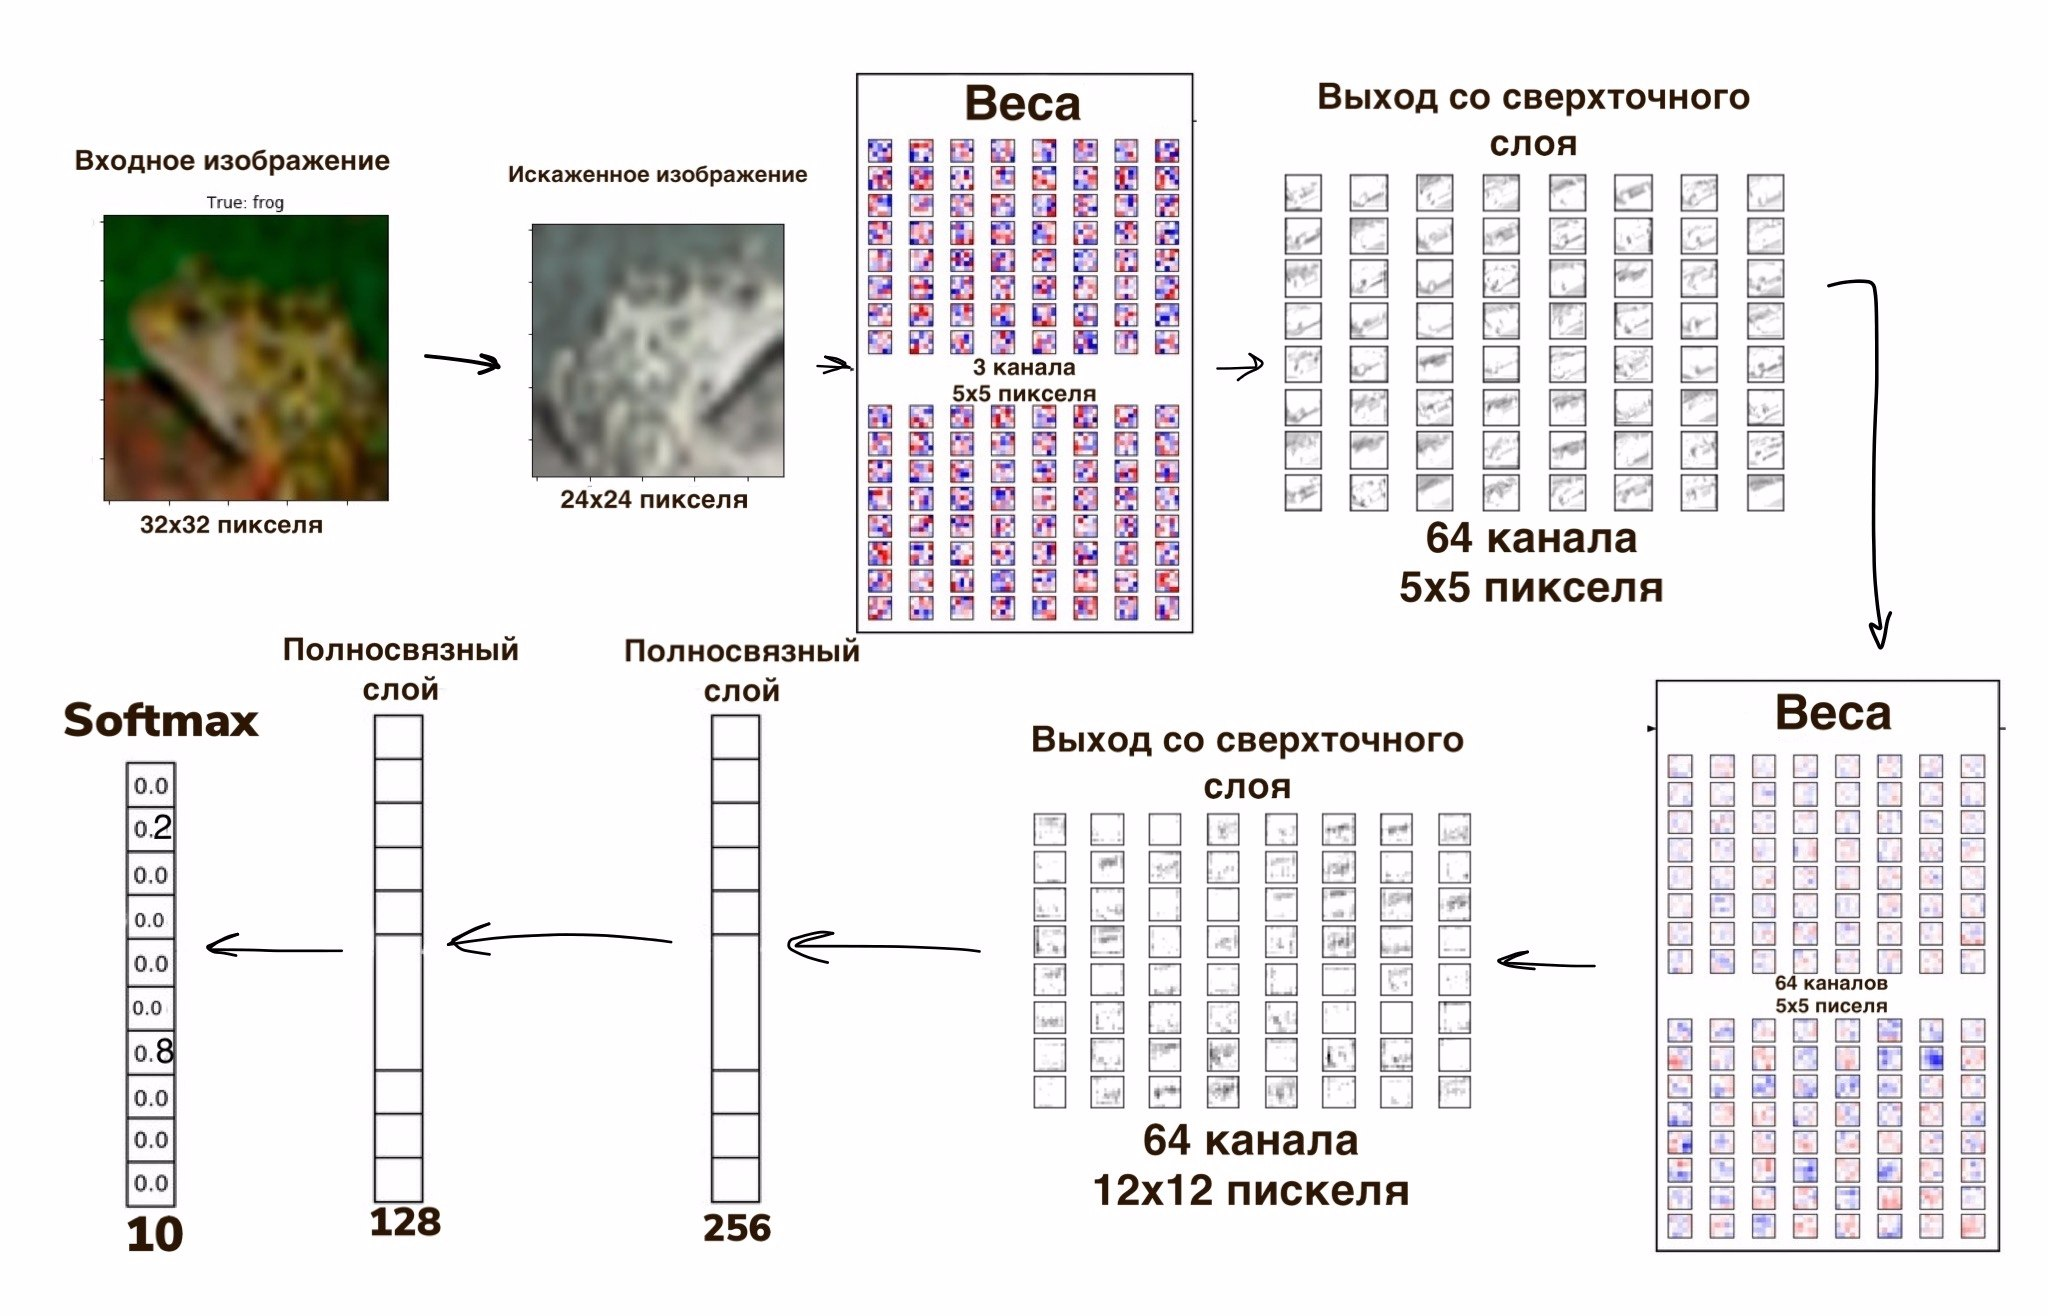
\includegraphics[width=0.9\textwidth]{fig/cnn_my.jpg}
	\caption{Структура сверточной нейронной сети}
	\label{SRTCT}
\end{figure}

На рисунке  \ref{fig:SRTCT}  показана структура нейронной сети. Сначала каждое изображение проходит через функцию искажения. Затем сеть будет состоять из двух сверточных слоев и слоев субдискретизации. После этого выходное изображение слоя подвыборки трансформируется в одномерный вектор (слоем Flatten) и проходит два полносвязных слоя. На всех слоях, кроме выходного полносвязного слоя, используется функция активации ReLU, последний же слой использует softmax.


ReLU - простой выпрямитель, который имеет формулу  $$f(x) = max(0, x)$$. 
Softmax используется для того, что бы преобразовать вектор со второго полносвязного слоя в массив из 10 чисел (= количеству классов) с вероятностными значениями принадлежности к классу, которые в сумме дали бы 1.


\subsubsection{Структура сети}

Функция случайного искажения изображения, принимает на вход изображение из набора данных CIFAR и случайно обрезает, переворачивает, изменяет контраст, яркость, насыщенность и оттенок. Это делается для того, чтобы искусственно увеличить объем выборки.

Результат показан на картинке  \ref{fig:DISORT}. Слева представлена картинка с набора данных CIFAR, справа 9 разных искаженных изображений.

\begin{figure}[htbp]
	\centering
	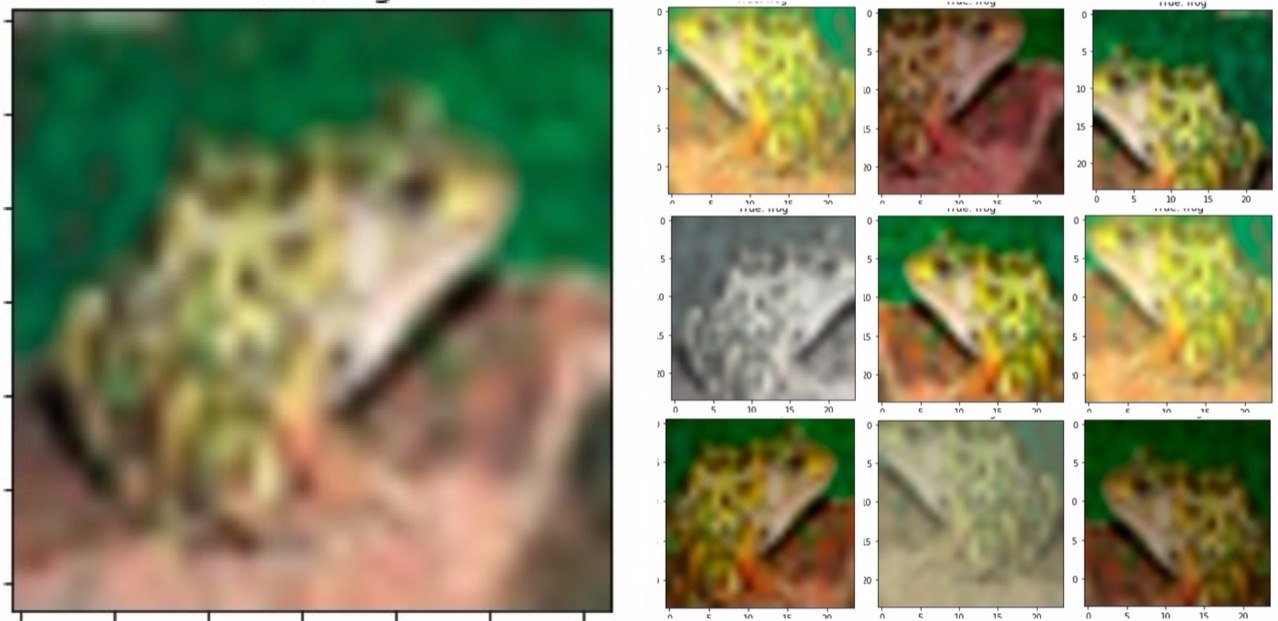
\includegraphics[width=0.7\textwidth]{fig/disort.jpg}
	\caption{Пример работы функции "distort_image"}%
	\label{fig:DISORT}
\end{figure} 


Сеть имеет следующие параметры:
\begin{itemize}
\item batch size = 32— количество обучающих образцов, обрабатываемых одновременно за одну итерацию алгоритма градиентного спуска;
\item num epochs = 1000 — количество итераций обучающего алгоритма по всему обучающему множеству;
\item kernel size = 5 — размер ядра в сверточных слоях;
\item pool size = 2 — размер подвыборки в слоях подвыборки;
\item depth = 64 — количество ядер в сверточных слоях;
\item fc size1 = 256 — количество нейронов в 1ом полносвязном слое;
\item fc size2 = 128.
\end{itemize}

При большом количестве итераций обучение может занять много времени, если обучать сеть без использования графического процессора. Поэтому в учебник был добавлен Saver. Saver может сохранять переменные в контрольные точки.  Также он может найти последнюю контрольную точку и достать из нее переменные.

Таким образом процесс обучения можно отложить, а затем снова начать не потеряв результата.


В качестве функции потерь используется кросс-энтропия.

Модель достигает точности около 90 процентов на тестовом множестве, учитывая относительную простоту модели, это вполне достойный результат. 

\subsubsection{Варианты}
Студентам предлагается выбрать себе набор данных из 15-ти представленных (Fashion-MNIST, Caltech-256, Linnaeus 5 и другие) и обучить сеть, опираясь на уже представленный код. В отчете построить и проанализировать веса и выходы с сверточных слоев.






\subsection{Реализация второй лабораторной работы}
Во второй лабораторной работе студентам предлагается создать свой набор данных и переобучить существующую модель глубокого обучения для задачи детектирования объектов, используя Tensorflow Object Detection API. 

\subsubsection{Введение}

Первая часть работы заключается в том, чтобы показать как подключить и запустить уже существующую замороженную модель для локализации объектов. Во второй части предстоит собрать изображения, промаркировать их, разделить изображения на изображения для тренировки и теста, создать tfrecords для обеих выборок, настроить .config-файл , переобучить сеть, создать граф модели и протестировать на тестовой выборке.

Tensorflow Object Detection API - это платформа с открытым исходным кодом, созданная на основе TensorFlow. Она содержит несколько моделей машинного обучения, способных локализовать и классифицировать несколько объектов на одном изображении. Модели обучались на таких наборах данных как: COCO,  Kitti и  Open Images.

Модель для демонстрирования примера - ssd mobilenet v1 coco, так как она самая быстрая из представленных. Она использует алгоритм - Single Shot detectors \cite{SSD}.

\subsubsection{Варианты}
В качестве вариантов, предлагается выбрать объект, которого нет в словаре сети и переобучить модель.












\subsection{Реализация третьей лабораторной работы}

В этом примере показано, как прогнозировать данные временных рядов с использованием сети с длинной короткосрочной  памятью (LSTM).

Чтобы прогнозировать значения будущих шагов времени последовательности, достаточно обучить сеть LSTM с последовательной регрессией, где ответы представляют собой обучающие последовательности со значениями, сдвинутыми на один временной шаг. То есть на каждом временном шаге входной последовательности сеть LSTM учится прогнозировать значение следующего шага времени.

В этом примере используется набор данных "monthly milk production pound". Набор охватывает период с января 1962 года по декабрь 1975 и содержит информацию о количестве произведенного молока в месяц коровой.

\begin{figure}[htbp]
	\centering
	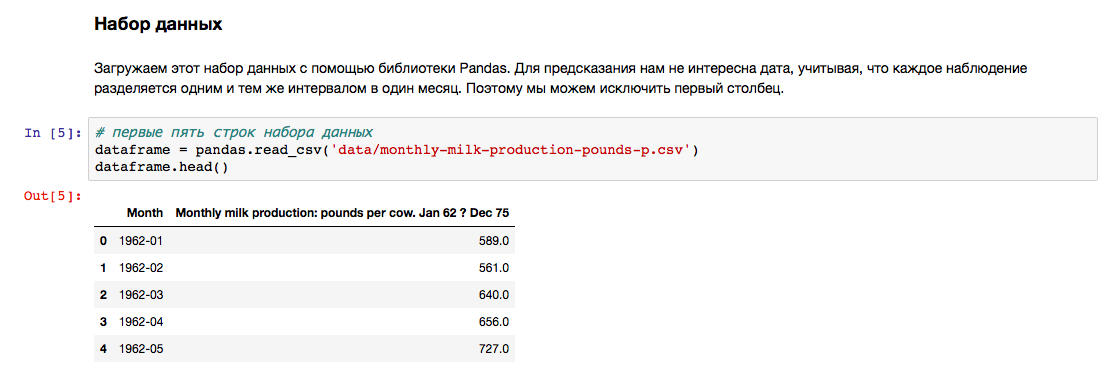
\includegraphics[width=0.7\textwidth]{fig/milk}
	\caption{Структура нейронное сети}%
	\label{fig:milk}
\end{figure}


Пример обучает сеть LSTM прогнозировать количество молока, которое может произвести корова, учитывая ее предыдущие показатели.

Данные были разделены на тренировочный и тестовый набор в соотношении 90/10.

LSTM состоит из двух скрытых слоев, на первом -14 нейронов, на втором - 8 и выходным слоем. Функция активации relu, оптимизатор использует метод стохастических градиентов.

Среднеквадратичная ошибка составила 43.45 единиц  для тренировочного набора и 45.4 единиц для тестового.


\begin{figure}[htbp]
	\centering
	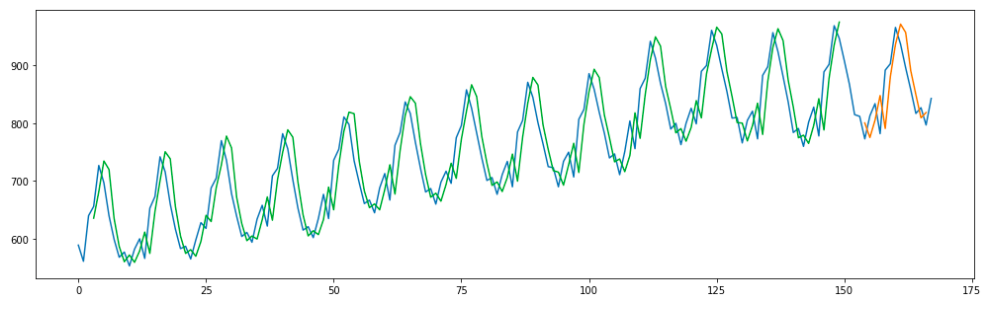
\includegraphics[width=0.7\textwidth]{fig/predict}
	\caption{Структура нейронное сети}%
	\label{fig:predict}
\end{figure}


\subsubsection{Варианты}
В качестве вариантов предлагается студентам выбрать набор данных и сделать предсказания. Попытаться, варьируя количество нейронов в слоях, количество слоев и количество эпох - минимизировать ошибку.


